\section{An Exploration into Various Neural Architectures for the Simulator Replacement}\label{Appendix:Networks}

Recall that ARAMNet (\Cref{table:simple-network}) is a very simple network consisting of a single layer of LSTM cells followed by a single linear layer.
As such, most of our exploration will be focussed on various deep versions of this.

We start with two natural deep versions of ARAMNet.
Network 2 (\Cref{Table:Network-2}) extends the number of LSTM layers, while Network 3 (\Cref{Table:Network-3}) extends the number of Linear layers.
Next, we treat ARAMNet as its own module (without the final softmax layer).
Stacking ARAMNet modules one after another gives us Network 4 (\Cref{Figure:Network-4}).
Finally, we out something really funky.
Taking inspiration by the law of total probability, we wanted to help the neural network learn that type of formula.
As such Network 5 (\Cref{Figure:Network-5}) does exactly this and perform additions and multiplications on the outputs of ARAMNet modules. 

\begin{table}[htbp]
    \centering\small
    \begin{minipage}{.49\textwidth}
        \centering
        \begin{tabular}{|c|c|c|c|}
            \hline
            Layer            & \makecell{Kernel \\ Shape} & \makecell{ Output \\ Shape} & \# Params \\
            \hline
            \makecell{LSTM \\ (3 layers)}  &              & (10, 152)    & ${\sim}558$k  \\
            \hline 
            Flatten          &              & (1, 1520)    &           \\ 
            \hline
            Linear           & (1520, 1520) & (1, 1520)    & ${\sim}2$M  \\ 
            \hline
            Reshape          &              & (10, 152)    &           \\ 
            \hline
            Softmax          &              & (10, 152)    &           \\ 
            \hline
        \end{tabular}
        \label{Table:Network-2}
        \caption{Network 2 Architecture (We omit the BatchNorm layer and Dropout layers between the individual LSTM layers)}
    \end{minipage}\hfill
    \begin{minipage}{.49\textwidth}
        \centering
        \begin{tabular}{|c|c|c|c|}
            \hline
            Layer             & \makecell{Kernel \\ Shape} & \makecell{Output \\ Shape} & \# Params   \\
            \hline
            LSTM              &              & (10, 152)    & ${\sim}184$k    \\
            \hline 
            Flatten           &              & (1, 1520)    &             \\ 
            \hline
            {\footnotesize \makecell{Linear \\ (3 Layers)}} & (1520, 1520) & (1, 1520)    & ${\sim}7$M  \\ 
            \hline
            Reshape           &              & (10, 152)    &             \\ 
            \hline
            Softmax           &              & (10, 152)    &             \\ 
            \hline
        \end{tabular}
        \label{Table:Network-3}
        \caption{Network 3 Architecture (We omit the BatchNorm, Dropout and Activation layers between each Linear layer)}
    \end{minipage}
\end{table}

\begin{figure}[htbp]
    \centering\small
    \begin{tikzpicture}
        \node[shape=rectangle, draw, thick] (1) at (0, 0) {ARAMNet};
        \node[shape=rectangle, draw, thick] (2) at (3, 0) {ARAMNet};
        \node[shape=rectangle, draw, thick] (3) at (6, 0) {ARAMNet};
        \node[vertex] (s) at (9, 0) {Softmax};
        \node[vertex] (out) at (11, 0) {$\hat{y}$};

        \draw[edge] (1) to (2);
        \draw[edge] (2) to (3);
        \draw[edge] (3) to (s);
        \draw[edge] (s) to (out);
    \end{tikzpicture}
    \label{Figure:Network-4}
    \caption{Network 4 Architecture Diagram}
\end{figure}

\begin{figure}[htbp]
    \centering\small
    \begin{tikzpicture}[scale=0.5]
        \node[shape=rectangle, draw, thick] (1) at (0, 0) {ARAMNet};
        \node[shape=rectangle, draw, thick] (2) at (0, -4) {ARAMNet};
        \node[shape=rectangle, draw, thick] (3) at (0, -8) {ARAMNet};
        \node[shape=rectangle, draw, thick] (4) at (12, -6) {ARAMNet};
        \node[vertex] (+) at (3, -2) {$+$};
        \node[vertex] (*) at (6, -6) {$*$};
        \node[vertex] (s) at (17, -6) {Softmax};
        \node[vertex] (out) at (20, -6) {$\hat{y}$};

        \draw[edge, to path={-| (\tikztotarget)}] (1) to (+);
        \draw[edge, to path={-| (\tikztotarget)}] (2) to (+);
        \draw[edge, to path={-| (\tikztotarget)}] (+) to (*);
        \draw[edge, to path={-| (\tikztotarget)}] (3) to (*);
        \draw[edge] (*) to (4);
        \draw[edge] (4) to (s);
        \draw[edge] (s) to (out);
    \end{tikzpicture}
    \label{Figure:Network-5}
    \caption{Network 5 Architecture Diagram}
\end{figure}

We trained the 4 networks on our small validation dataset of $300$ randomly generated samples, using the default settings for Adam and a batch size of 32, and plotted their learning curves alongside ARAMNet in \Cref{Figure:Training-Loss-All-Networks}.
Network 2 and (intriguingly) Network 5 were also considered as candidates to replace the simulator function.
In particular, we were very surprised that Network 5 achieved a loss matching ARAMNet.
It is, in fact, learning something interesting about the data and not just memorizing it, since the network contains ${\sim}9$ million parameters, yet, Network 3 with ${\sim}7$M performs \it{much} worse.

\begin{figure}[htbp]
    \centering
    \begin{minipage}{\textwidth}
        \centering
        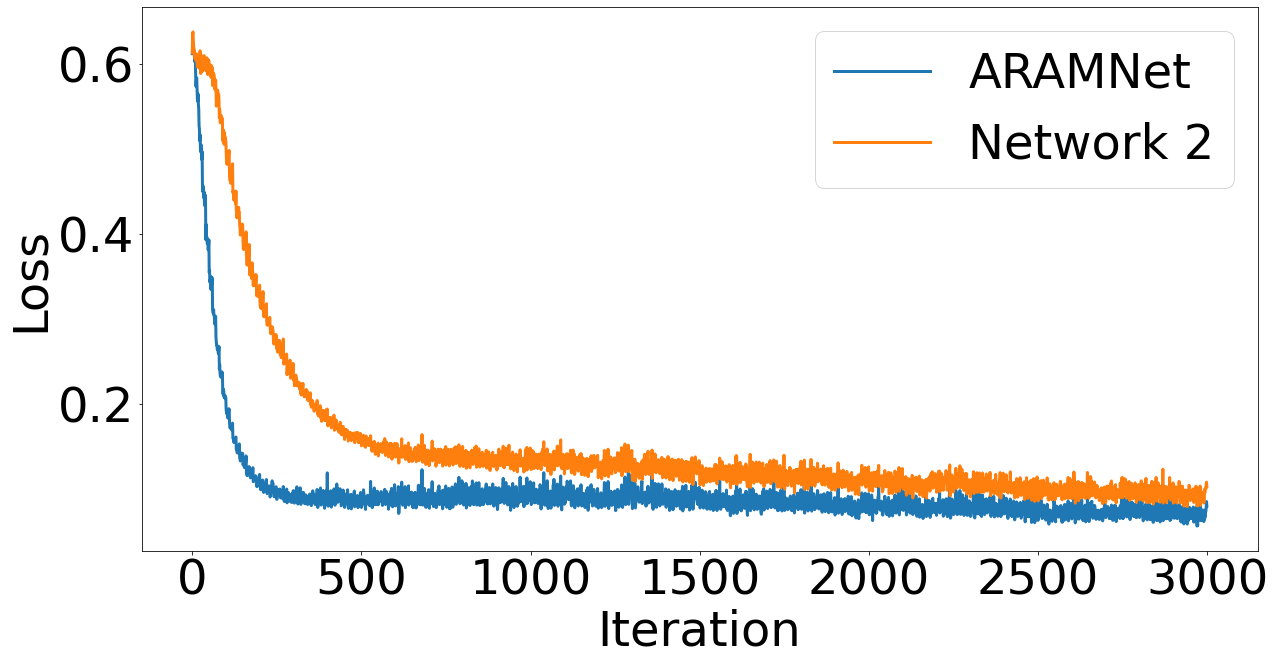
\includegraphics[width=.49\textwidth]{figures/explore-val-loss/network-2.png}\hfill
        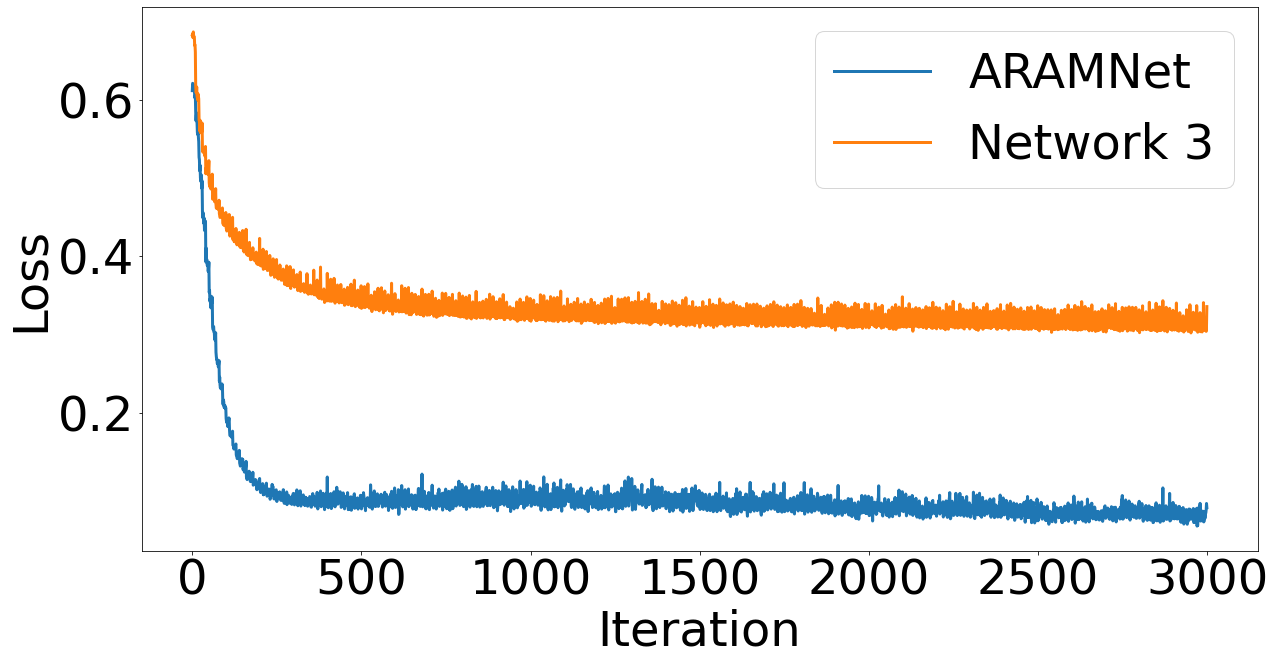
\includegraphics[width=.49\textwidth]{figures/explore-val-loss/network-3.png}
    \end{minipage}\hfill
    \vspace{3mm}
    \begin{minipage}{\textwidth}
        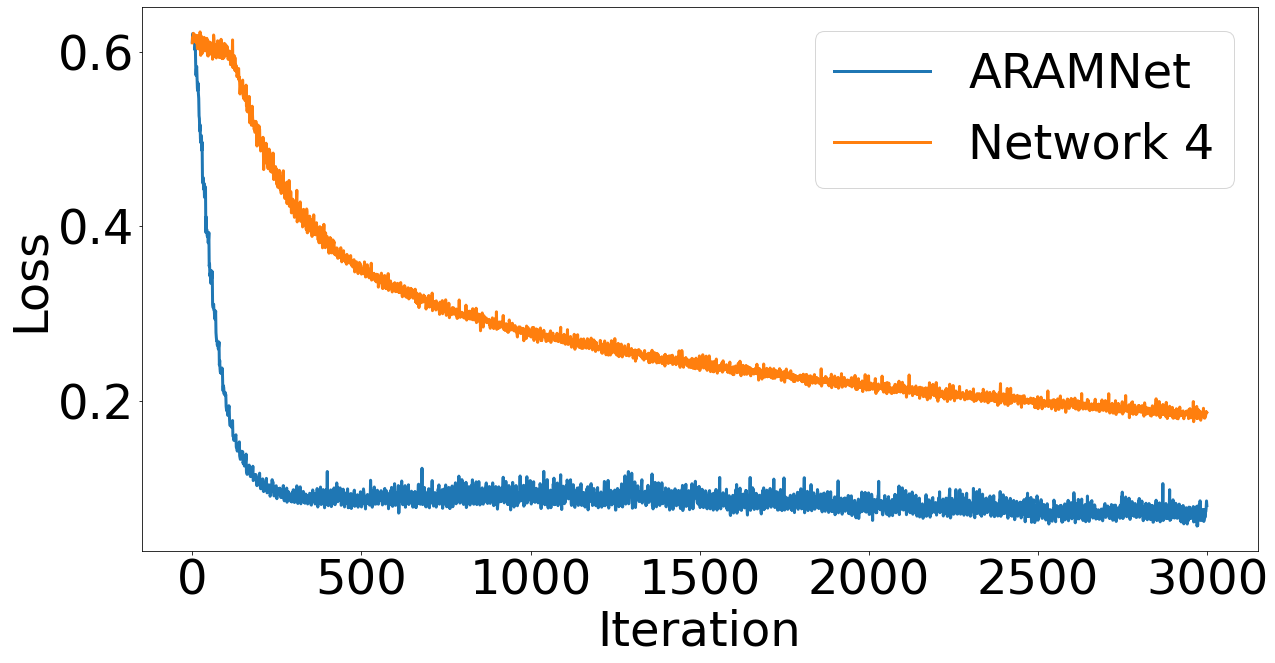
\includegraphics[width=.49\textwidth]{figures/explore-val-loss/network-4.png}\hfill
        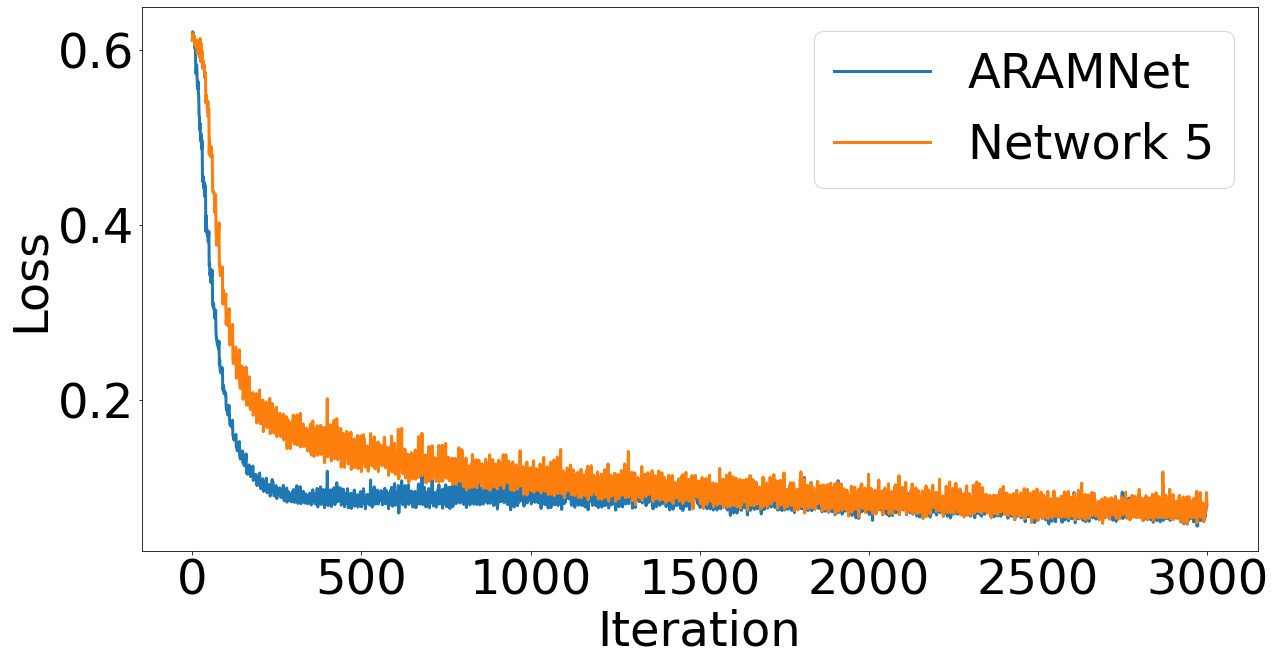
\includegraphics[width=.49\textwidth]{figures/explore-val-loss/network-5.png}
    \end{minipage}
    \label{Figure:Training-Loss-All-Networks}
    \caption{Learning Curve of the 4 alternate networks compared to the learning curve of ARAMNet on the validation dataset}
\end{figure}

However, these two networks were more difficult to train and we had trouble preventing them from overfitting.
Although they could reach training losses matching that of ARAMNet, their validation loss were much too high for them to be useful simulator replacement candidates
In \Cref{Figure:Training-Loss-2-and-5}, we can see just how large the training-to-validation loss gap is, as compared to \Cref{Figure:ARAMNet-Learning-Curve}.

\begin{figure}
    \centering
    \begin{minipage}{\textwidth}      
        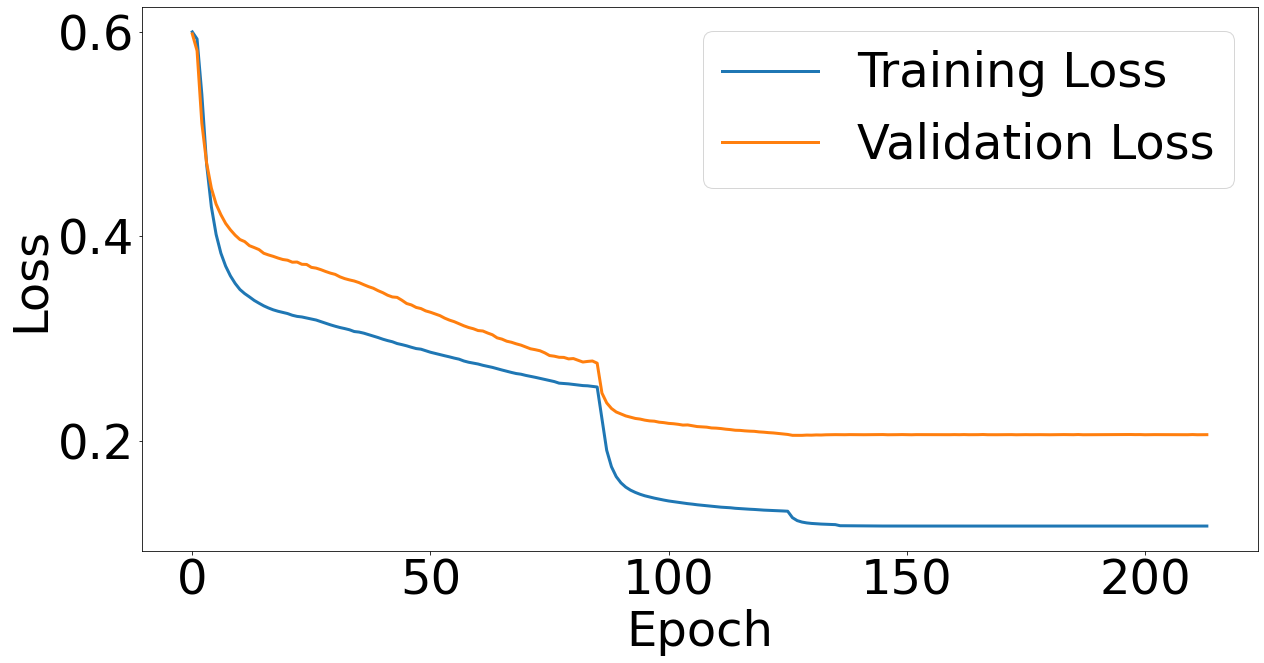
\includegraphics[width=.49\textwidth]{figures/explore-train-loss/network-2.png}\hfill
        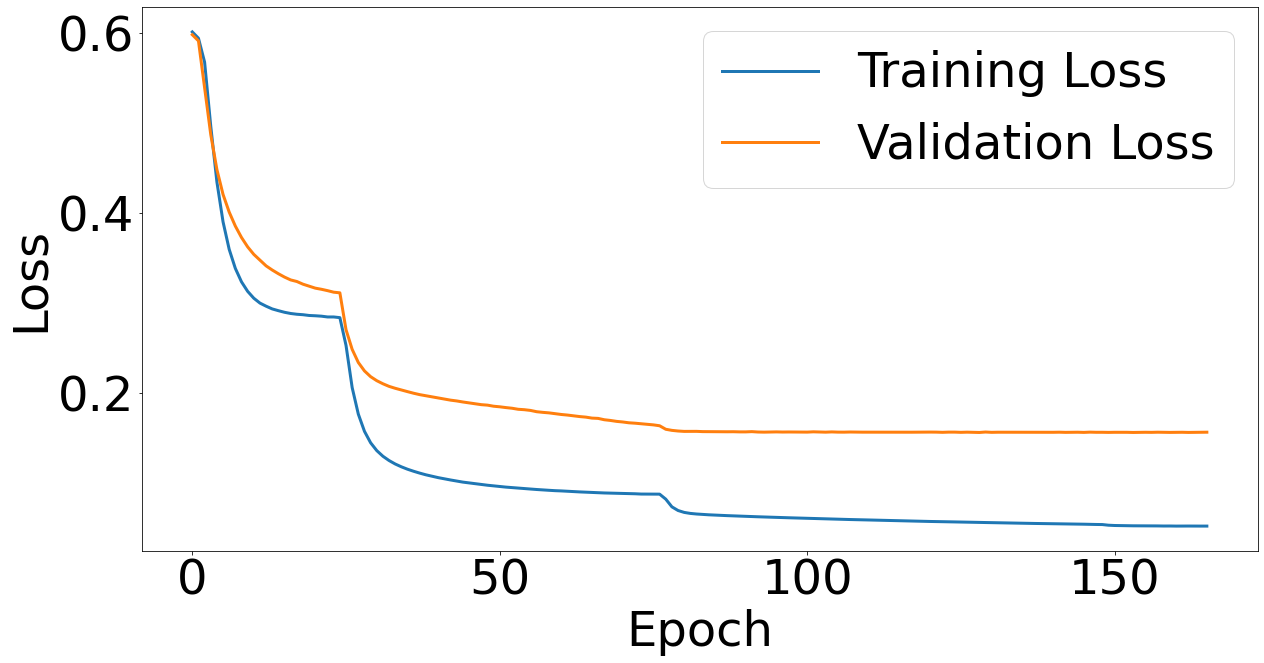
\includegraphics[width=.49\textwidth]{figures/explore-train-loss/network-5.png}
    \end{minipage}
    \label{Figure:Training-Loss-2-and-5}
    \caption{Learning curves for Networks 2 and 5 when we trained using the same optimizer and settings as with ARAMNet.}
\end{figure}